
\chapter{Background \& Literature review}

In order to meet our goal, necessary knowledge on phishing in general
is required. This chapter introduces general understanding of phishing,
an exploration of its damage in term of money, the overview of its
modus operandi, a brief explanation on types of phishing, general
phishing countermeasures and human factor in phishing attacks.


\section{What is phishing?}

While the Internet has brought convenience to many people for exchanging
information, it also provides opportunities to carry malicious behavior
such as online fraud on massive scale with a little cost to the attackers.
The attackers can manipulate the Internet users instead of computer
system (hardware or software) that significantly increase the barriers
of technological crime impact. Such human centered attacks could be
done by social engineering. According to Jakobsson, et al. phishing
is a form of social engineering that aim{\small{}s} to retrieve credential
from online users by mimicking trustworthy and legitimate institutions
\citep{jakobsson:2006}. Phishing has a similar basic principle as
\textquoteleft fishing\textquoteright{} in the physical world. Instead
of fish, online users are lured by authentic looking communication
and hooked by authentic looking websites. Not only that, online users
also may be lured by respond to a phishing email, either replying
or clicking a hidden URL within its content. There are diverse definitions
of phishing in our literature reviews, therefore, we would like to
discuss about its universal definition in later section. However,
one of phishing definitions according to Oxford dictionary:
\begin{quote}
``A fraudulent practice of sending emails purporting to be from reputable
companies in order to induce individuals to reveal personal information,
such as passwords and credit card numbers, online'' \citep{oxford}. 
\end{quote}
\begin{onehalfspace}
Several studies suggest that phishing is a form of online criminal
activity by using social engineering techniques \citep{jakobsson:2006}\citep{workman:2008}\citep{jagatic2007social}\citep{chandrasekaran:2006}.
An individual or a group who uses this technique is called \emph{Phisher(s}).
After successfully obtained a sensitive information from the victim,
phishers use this information to access victim\textquoteright s financial
accounts or committing credit card frauds. However, to formalize the
damage of phishing in term of money is a challenging task. We will
briefly explore the cost of phishing attacks in the later section. 
\end{onehalfspace}

Furthermore, the technique or modus operandi of phishing may vary,
but the most common technique of phishing attacks done by using fraudulent
emails and websites \citep{james:2005}. A fraudulent website is designed
in such a way that it may be identical to its legitimate target. While
it may be true, phishing website also could be completely different
with its target as there is no level of identicalness. In the following
subsections, we will introduce how phishing was originally came about
and how current literatures formally define phishing.


\subsection{The History }

The first time the term \textquotedbl{}phishing\textquotedbl{} was
published by the \ac{AOL} UseNet Newsgroup on January 2, 1996 and
was started to expand in 2004 \citep{phishorg}. Since then, we considered
phishing development in cyberspace has been flourishing by phishers
to make profit. Total losses due to phishing in 2004 reached more
than U.S. \$ 2 billion, it was involving more than 15,000 sites that
become victims \citep{fellman:2004}. We will try to discuss about
direct and indirect cost at present days in the later section. Evidently,
Jakobsson, et al. \citep{jakobsson:2006} mentioned that in the early
years of 90\textquoteright s (according to \citep{phishorg} it was
around 1995) many hackers would create bogus AOL user accounts with
automatically generated fraudulent credit card information. Their
intention to give this fake credit card information was to simply
pass the validity tests performed by AOL. By the time the tests were
passed, AOL was thinking that these accounts were legitimate and resulted
to activate them. Consequently, these hackers could freely access
AOL resources until AOL tried to actually bill the credit card. AOL
realized that these accounts were using invalid billing information,
thus deactivated the account. 

While creating false AOL user accounts with fake credit card information
was not exactly phishing attacks, but AOL\textquoteright s effort
to counter against the attacks was leading to development of phishing.
This countermeasure includes directly verifying the legitimacy of
credit card information and the associated billing identity, forced
hackers to pursue alternative way \citep{jakobsson:2006}. Hackers
were masquerading as AOL\textquoteright s employees asking to other
users for credit card information through AOL instant messenger and
email system \citep{phishorg}. Jakobsson et al. suggest that phishing
attacks were originating from this incident \citep{jakobsson:2006}.
Since such attack has not been done before, many of users have been
victimized by then. Eventually, AOL enforced warning system to the
most of its customers to be vigilant when it comes to sensitive information
\citep{phishorg}. At the present day, phishing attacks might not
only being motivated by financial gain but also political reason,
and they have been emerging not only aim to AOL users, but also any
online users. Consequently, large number of legitimate institutions
such as PayPal and eBay are being spoofed.


\subsection{The universal definition }

Before we begin to understand deeper about how and why phishing attack
works, we will briefly explore common phishing definition. Currently,
there is no consensus definition, since almost in every research papers,
academic textbook or journals has its own definition of phishing \citep{jakobsson:2006,james:2005,tally:2004,clayton:2005,parno:2006,jakobsson:2005,dhamija2006phishing}.
Phishing is also constantly evolving, so it might be very challenging
to define its universal terminology. There is not so much study that
specifically addresses the standard of phishing definition. However,
one research conducted by Lastdrager \citep{lastdrager:2014} addressed
to achieve consensual definition of phishing. Before we comply with
one consensual phishing terminology, we will take a look at various
phishing definitions from other sources:
\begin{quote}
``Phishing is the act of sending a forged e-mail (using a bulk mailer)
to a recipient, falsely mimicking a legitimate establishment in an
attempt to scam the recipient into divulging private information such
as credit card numbers or bank account passwords'' \citep{james:2005}

``Phishing is a form of Internet scam in which the attackers try
to trick consumers into divulging sensitive personal information.
The techniques usually involve fraudulent e-mail and websites that
impersonate both legitimate e-mail and websites'' \citep{tally:2004}

``Phishing is an attack in which victims are lured by official looking
email to a fraudulent website that appears to be that of a legitimate
service provider'' \citep{clayton:2005}

``In phishing, an automated form of social engineering, criminals
use the internet to fraudulently extract sensitive information from
business and individuals, often by impersonating legitimate websites''
\citep{parno:2006}
\end{quote}
It is noteworthy that the definition described by James, et al, Tally,
et al, and Clayton, et al. \citep{james:2005,tally:2004,clayton:2005}
specifies that the phishers only use email as a communication channel
to trick potential victims. While it might be true because using email
would greatly cost effective, but we believe that phishing is not
only characterized by one particular technological mean, as phishers
can also use any other electronic communication to trick potential
victims (i.e private message on online social network). This definition
is also similar to dictionary libraries \citep{oxford,collins,merriam}
that mention email as a medium communication between phishers and
users.

We believe that standard definition of phishing should be applicable
in most of phishing concept that are presently defined. Consequently,
the high level of abstraction and is required to build common definition
on phishing. We have convinced that the formal definition of phishing
should not focus on the technology that is being used but rather on
the technique how the deception is being conducted, the method of
an ``act'' if you will. Therefore, We follow the definition of phishing
by Lastdrager \citep{lastdrager:2014} which stated: 
\begin{quote}
\textit{``Phishing is a scalable act of deception whereby impersonation
is used to obtain information from a target''}
\end{quote}
According to Lastdrager \citep{lastdrager:2014}, to achieve this
universal definition, a systematic review of literature up to August
2013 was conducted along with manual peer review, which resulted in
113 distinct definitions to be analyzed. We thereby agree with Lastdrager
\citep{lastdrager:2014} that this definition addresses all the essential
elements of phishing and we will adopt it as universally accepted
terminology throughout our research.


\section{\label{sec:cost-of-phishing}The costs of phishing attacks}

It is a challenging task to find a real cost from phishing attacks
in term of money or direct cost. This due to financial damage for
bank is only known by banks and most institutions do not share this
information with the public. Evidently, Jakobsson et al. argue that
phishing economy is consistent with black market economy and does
not advertise its successes \citep{jakobsson:2006}. On this section,
a brief explanation of direct and indirect cost on phishing attack
will be illustrated based on literature review

According to Jakobsson et al., direct cost is depicted by the value
of money or goods that are directly stolen through phishing attack
\citep{jakobsson:2006}. While indirect cost is the costs that do
not represent the money nor goods that are actually stolen, but it
is the costs has to be paid by the people who handle these attacks
\citep{jakobsson:2006} (i.e. time, money and resources spent to reset
people password).

As we mentioned earlier, the difficulty of assessing the damage on
phishing attacks is caused by banks and institutions that keep this
information themselves and the unwillingness of many users to share
to acknowledge that they have been victimized by phishing attacks.
This happens because of fear of humiliation, financial loses, or legal
liability \citep{jakobsson:2006}. Evidently, studies estimate the
damage ranging from \$61 million \citep{herley:2009} to \$3 billion
per year \citep{mccall2007gartner} of direct losses to victims in
the US only \citep{hong:2012}\citep{moura2009scalable}. In addition,
the Gartner Group claimed to estimate of \$1.2 billion direct losses
of phishing attack to US banks and credit card companies for the year
2004 \citep{litan2004phishing}. By the 2007, it escalated to more
than \$3 billion loss \citep{mccall:2007}. The estimation also performed
by TRUSTe and Pontoon Institute that stated the cost of phishing attack
was up to \$500 millions losses in the US for the same year %
\footnote{http://wow.theregister.co.uk/2004/09/29/phishing\_survey/%
}.

However, the lack of information such as the detailed of documentation
survey on how to find these numbers which conducted by Gartner group
or Pontoon makes these estimations are biased than is generally realized.
It is interesting to investigate why their estimations are repeated
without really analyzed when they appeared biased at best. One thing
come up in our mind that they might have a hidden agenda to make societies
think that the cost of phishing is high. Consequently, people would
be obligated to implement anti phishing system or engage in phishing
awareness in their company which require money. With this in mind,
we would like to emphasize that our findings on the costs of phishing
attacks are only estimations without scrutiny from academic researchers
and it might be an exaggeration. Although even if the cost of phishing
attack is zero, we believe that phishing is still a major problem
in terms of trust among users and the misuse of email as a means of
communication.

Apart from the cost of phishing attacks, we might ask how phishing
attack is carried out? is there any stages involved? The next chapter
we will review its modus operandi in term of phishing stages or phases.


\section{Modus operandi}

As we mentioned earlier, Phishing attack is a subset of identity theft.
The modus operandi might be carried out firstly by creating a fake
website that spoofs legitimate website such as financial website,
either identical or not identical as long as the phishers get responds
from unsuspected victims. After that, the phishers will try to trick
the potential victim to submit important information such as usernames,
passwords, PINs, etc. through a fake website that they have created
or through email reply from victims. With the information obtained,
they will try to steal money from their victims if target institution
is a bank. Phishers employ variety of techniques to trick potential
victims to access their fraudulent website. One of the typical ways
is by sending illicit email in a large scale claiming to be from legitimate
institution. In the email content, they usually imitate an official-looking
logo, using good business language style and often also forge the
email headers to make it look like originating from legitimate institution.
For example, the content of the email is to inform the user that the
bank is changing its IT infrastructure, and request urgently that
the customer should update their data with the consequence of loosing
their money if the action does not take place. When the user click
the link that was on the email message, they will be redirected to
a fraudulent website, which will prompt the victim to fill in the
details of their information. While there are various techniques of
phishing attack, we will address the common phases of phishing that
we analyzed by literature survey by several studies and also we will
address our own phishing phases. These phases are compiled in \autoref{tab:compilation-phases}.

\begin{flushleft}
\begin{longtable}{|>{\raggedright}p{12cm}|}
\caption{\label{tab:compilation-phases}Compilation of phishing phases}
\tabularnewline
\hline 
J. Hong \citep{hong:2012}\tabularnewline
\hline 
{\scriptsize{}1. Potential victims receive a phish}{\scriptsize \par}

{\scriptsize{}2. The victim may take a suggested action in the message}{\scriptsize \par}

{\scriptsize{}3. The phisher monetizes the stolen information}\tabularnewline
\hline 
Frauenstein, et al. \citep{frauenstein:2013}\tabularnewline
\hline 
{\scriptsize{}1. Planning}{\scriptsize \par}

{\scriptsize{}2. Email Design}{\scriptsize \par}

{\scriptsize{}3. Fabricated story}{\scriptsize \par}

{\scriptsize{}4. Threatening tone/Consequences}{\scriptsize \par}

{\scriptsize{}5. Spoofed website}\tabularnewline
\hline 
Wetzel \citep{wetzel:2005}\tabularnewline
\hline 
{\scriptsize{}1. Planning}{\scriptsize \par}

{\scriptsize{}2. Setup}{\scriptsize \par}

{\scriptsize{}3. Attack}{\scriptsize \par}

{\scriptsize{}4. Collection}{\scriptsize \par}

{\scriptsize{}5. Fraud}{\scriptsize \par}

{\scriptsize{}6. Post-attack}\tabularnewline
\hline 
Tally, et al. \citep{tally:2004}\tabularnewline
\hline 
{\scriptsize{}1. The attacker obtains E-mail addresses for the intended
victims}{\scriptsize \par}

{\scriptsize{}2. The attacker generates an E-mail that appears legitimate}{\scriptsize \par}

{\scriptsize{}3. The attacker sends the E-mail to the intended victims
in a way that appears legitimate and obscures the true source}{\scriptsize \par}

{\scriptsize{}4. The recipient opens a malicious attachment, completes
a form, or visits a web site}{\scriptsize \par}

{\scriptsize{}5. Harvest and exploitation}\tabularnewline
\hline 
Emigh \citep{emigh:2005}\tabularnewline
\hline 
{\scriptsize{}1. A malicious payload arrives through some propagation
vector}{\scriptsize \par}

{\scriptsize{}2. The user takes an action that makes him or her vulnerable
to an information compromise}{\scriptsize \par}

{\scriptsize{}3. The user is prompted for confidential information,
either by a remote web site or locally by a Web Trojan}{\scriptsize \par}

{\scriptsize{}4. The user compromises confidential information}{\scriptsize \par}

{\scriptsize{}5. The confidential information is transmitted from
a phishing server to the phisher}{\scriptsize \par}

{\scriptsize{}6. The confidential information is used to impersonate
the user}{\scriptsize \par}

{\scriptsize{}7. The phisher engages in fraud using the compromised
information}\tabularnewline
\hline 
Nero et al. \citep{nero:2011}\tabularnewline
\hline 
{\scriptsize{}1. Preparation }{\scriptsize \par}

{\scriptsize{}2. Delivery of the Lure }{\scriptsize \par}

{\scriptsize{}3. Taking the Bait }{\scriptsize \par}

{\scriptsize{}4. Request for Confidential Information }{\scriptsize \par}

{\scriptsize{}5. Submission of Information }{\scriptsize \par}

{\scriptsize{}6. Collection of Data }{\scriptsize \par}

{\scriptsize{}7. Impersonation }{\scriptsize \par}

{\scriptsize{}8. Financial Gain}\tabularnewline
\hline 
\end{longtable}
\par\end{flushleft}

Based on the example scenario explained earlier, phishing attacks
may consist of several phases. J. Hong \citep{hong:2012} argued that
there are three major phases. while Frauenstein, et al. \citep{frauenstein:2013}
suggested that there are five main processes are used to perform phishing
attacks based on the perspective of the attacker.

\begin{figure}
\begin{centering}
\includegraphics[scale=0.5]{\string"gfx/phishing processes\string".png}
\par\end{centering}

\protect\caption{\label{fig:frauenstein}Phishing processes based on Frauenstein\citep{frauenstein:2013}}
\end{figure}


As we illustrated in \autoref{fig:frauenstein}, on the first process
is called \textit{Planning}, a phisher usually would do some reconnaissance
on how would the attack is executed and what information would be
obtained from the victim. On the second process, the phisher would
think about the design of the email. This email is desired by the
phisher to look as legit as possible to potential victim. For this
purpose, target institutions logo, trademark, symbol, etc. are used
to make the content look official to the victim. The author called
this process as \textit{Email Design}. \autoref{fig:ing} illustrates
the example design of a fake email that impersonates ING bank that
can trick unsuspecting victims%
\footnote{http://wow.martijn-onderwater.nl/wp-content/uploads/2010/03/ing-phishing.jpg%
}. From the figure, we can spot a fake email by investigating the real
sender email address by looking at the email header or the URL provided
in the body, whether it redirects to the official ING website or not.
On the third process, the phisher \textit{fabricates} a story to make
potential victim think that email is important. To achieve users attention,
phisher might build up a story about system upgrade, account hijacked
or security enhancement so that the victim would feel obliged to be
informed. Evidently, this technique corresponds with Cialdini \citep{cialdini:2001}
that suggests there are six principles to persuade people to comply
with a request. On the fourth process, a phisher usually include \textit{threatening
tone} or explain the urgency and consequences if the potential victim
chooses not to take action desired by the phisher (for example; account
removal, account blocked, etc.). Consequently, users may fear of their
account being deleted. The last process involved with fraudulent website
that has been created by the phisher. Users may falsely believe to
the message given in the email and may click a \ac{URL} that is embedded
in the email. Subsequently, the URL would redirect users to a \textit{spoofed
website} which may prompt users\textquoteright{} sensitive information.
Furthermore, the website might be created to be as similar as possible
to the target institution\textquoteright s website, so that potential
victim may still believe that it is authentic. We will explain more
on Cialdini\textquoteright s six basic tendencies of human behavior
in generating positive response to persuasion \citep{cialdini:2001}
in a later section.

\begin{figure}
\begin{centering}
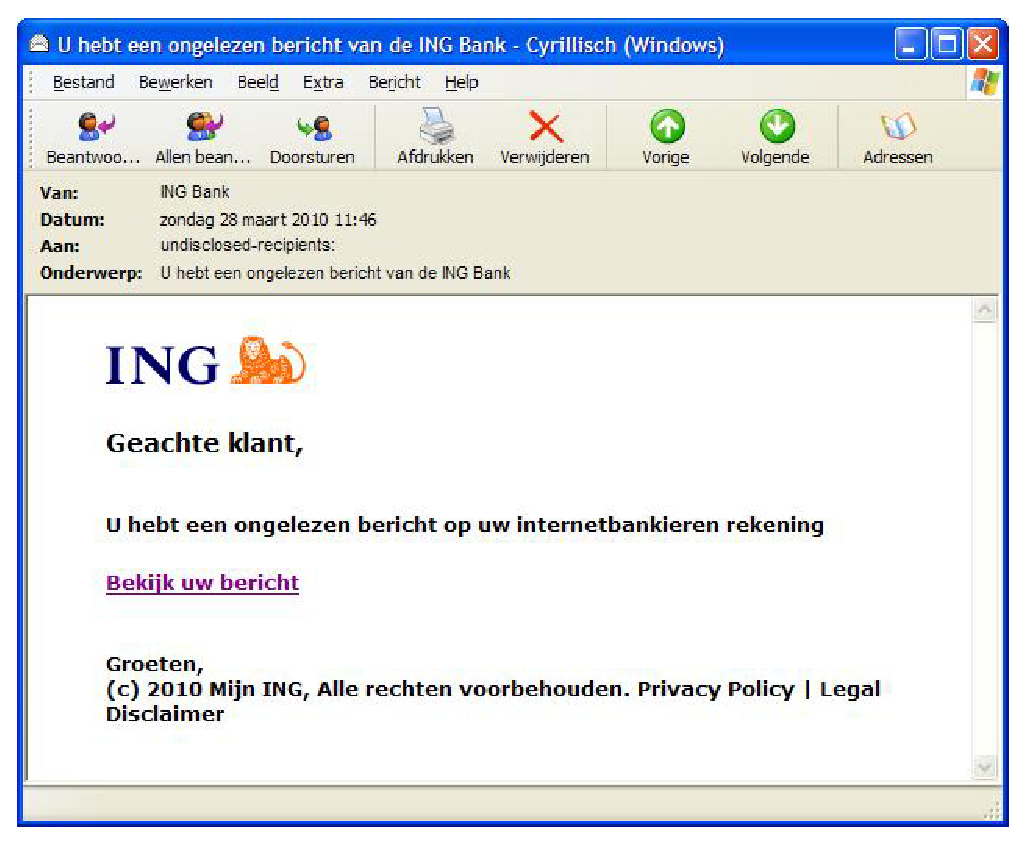
\includegraphics[scale=0.4]{gfx/ing-phishing}
\par\end{centering}

\protect\caption{\label{fig:ing}Example of a phishing email impersonating ING bank}
\end{figure}


Considering that phishing attack is a process, Wetzel \citep{wetzel:2005}
suggested a taxonomy to make sense of the complex nature of the problem
by mapping out a common attacks lifecycle, and a possible set of activities
attackers engage in within each phase. The taxonomy is illustrated
in \autoref{fig:wetzel}. We speculated that Wetzel's taxonomy is
not analogous with Frauenstein's main phishing processes \citep{frauenstein:2013}.
The difference is that Frauenstein et al. only focus in the design
of the attack while Wetzel has added several phases like \textit{Collection},
\textit{Fraud} and \textit{Post-attack}, therefore, Wetzel taxonomy
is more holistic in term of phishing.

\begin{figure}
\centering{}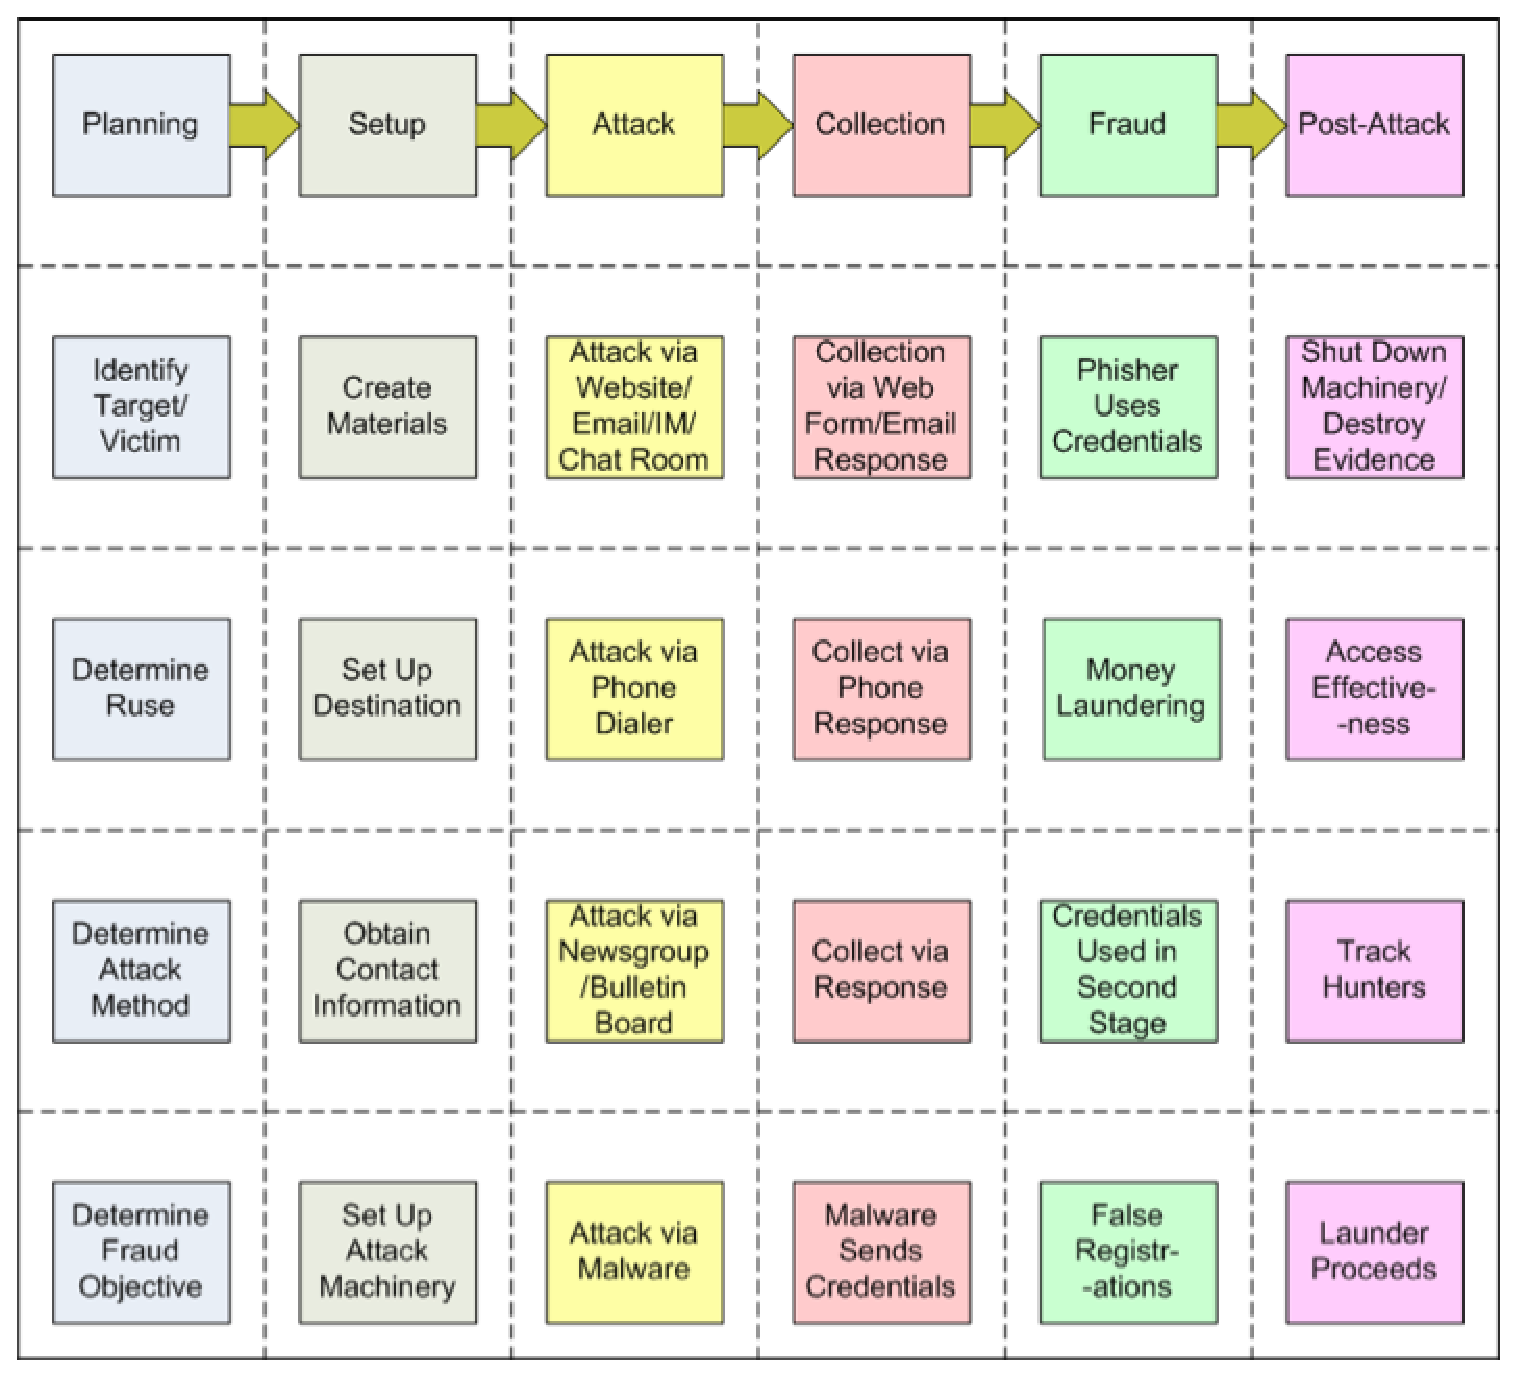
\includegraphics[scale=0.4]{gfx/wetzel}\protect\caption{\label{fig:wetzel}Phishing attack taxonomy and lifecycle\citep{wetzel:2005}}
\end{figure}


As we listed Wetzel's taxonomy in \autoref{tab:compilation-phases},
we explain more of the taxonomy as follows:
\begin{enumerate}
\item \textit{Planning}: Preparation carried out by the phisher before continue
to the next phase. Example activities include identifying targets
and victims, determine the method of the attack, etc.
\item \textit{Setup}: After the target, victim and the method are known,
the phisher would craft a platform where the victim's information
could be transmitted and stored, for example: fraudulent website/email.
\item \textit{Attack}: Phisher distributes their fraudulent platform so
that it can be delivered to the potential victims with fabricated
stories.
\item \textit{Collection}: Phisher collects valuable information via response
from the victims
\item \textit{Fraud}: Phisher abuses victim's information by impersonates
the identity of the victim to the target. For example, A has gained
B's personal information to access C so that A can pose as B to access
C.
\item \textit{Post-attack}: After the phisher gained profit from the attack
and abuse phases, a phisher would not want to be noticed or detected
by authority. Thus, phisher might need to destroy evidence of the
activities that he/she previously were executed.
\end{enumerate}
As shown in \autoref{tab:compilation-phases}. Tally, et al. suggest
that there are several phases involved in phishing attack based on
the attacker's point of view \citep{tally:2004}. The first phase,
it represents the planning, as we understand the attacker collects
the email address of unsuspecting victims. The second phase, considering
that it is related to creating a fake email that appears legitimate,
this phase can be viewed as design phase. On the third phase, we consider
this as delivery and attack phases as it involves the attacker sends
the fake email to the unintended victims and hide the true source.
The fourth phase represents attack phase as it involves with the recipient
complies with the attacker's request(s). Lastly the fifth phase, it
represents the fraud phase, as it related to haversting and exploiting
victim's resources by the attacker. Additionally, the phases described
by Tally, et al. \citep{tally:2004} are comparable with the information
flow explained by Emigh\citep{emigh:2005} illustrated in \autoref{fig:emigh}
and explained in \autoref{tab:compilation-phases}. Phishing attack
steps that executed by the phisher are also being addressed by Nero,
et al \citep{nero:2011}. In their study, a successful phishing attack
involves several phases which can bee seen and compare in \autoref{tab:compilation-phases}.

\begin{figure}
\begin{centering}
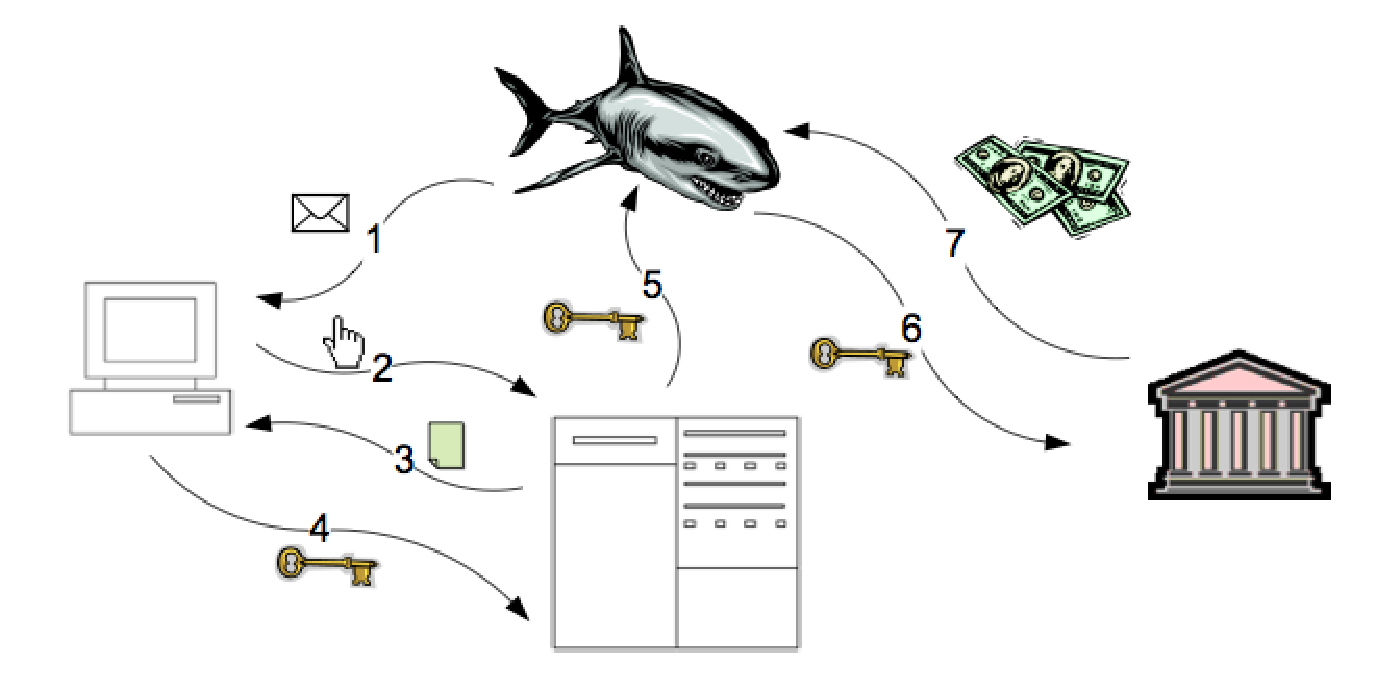
\includegraphics[scale=0.4]{gfx/emigh}\protect\caption{\label{fig:emigh}Flow of information in phishing attack \citep{emigh:2005}}

\par\end{centering}

\end{figure}


Based on our analysis by looking at the pattern of other phases from
various sources, there is a major similarity between them. Therefore,
we would like to define and design our own phase that are integrated
with three key components suggested by Jakobsson, et al. \citep{jakobsson:2006}.
These key components are include \textit{the lure},\textit{ the hook}
and \textit{the catch}. As we designed in \autoref{fig:Information-flow-phishing},
we synthesized these three components with our phases based on the
attacker point of view as follows:

- The lure 

1. Phishers prepare the attack 

2. Deliver initial payload to potential victim 

3. Victim taking the bait

- The hook 

4. Prompt for confidential information

5. Disclosed confidential information 

6. Collect stolen information 

- The catch

7. Impersonates victim 

8. Received pay out from the bank 

\begin{figure}
\centering{}Collect stolen information \includegraphics[scale=0.3]{gfx/info-flow-nolie}\protect\caption{\label{fig:Information-flow-phishing}Information flow phishing attack}
\end{figure}


It is important to know that in the phase 3, there are different scenarios
such as; victim might be redirected to a spoofed website, victim may
comply to reply the email, victim may comply to open an attachment(s)
or victim may comply to call by phone. However, in \autoref{fig:Information-flow-phishing},
we have only illustrated the phases if the bait was using a spoofed
website as a method. 

We have reviewed various phases in phishing attack and from the review,
we have constructed our own phases. In the next section, a brief introduction
in respect to the types of phishing will be described. We believe
that the general understanding of phishing types will help our main
analysis to characterize phishing email properties.


\section{Types of phishing}

In January 2014, 8300 patients data are being compromised in medical
company in the US \citep{adam:2014}. The data includes names, addresses,
date of birth and phone numbers were being stolen. Other than demographic
information, clinical information associated with this data was also
stolen, including social security numbers. In the April 2014, phishers
have successfully stolen US\$163,000 from US public school based on
Michigan \citep{ashley:2014}. It has been said that the email prompted
to transfer money is coming from the finance director of the school.
In March 2014, Symantec has discovered phishing attack aimed at Google
drive users \citep{teri:2014}. The attack was carried firstly with
incoming email asking for opening document hosted at Google docs.
Users that have clicked on the link are taken to fraudulent Google
login page prompted Google users credentials. Interestingly, the URL
seems very convincing because it hosted on Google secure servers.
We hypothesized that even more phishing incidents on financial area
as well, but sometimes the news is kept hidden due to creditability
reason. With this in mind, we believe fake websites might be hosted
in the network which has more phishing domain than other networks.
Subsequently, in the next section, we will discuss the general phishing
countermeasures. 

One may ask, what type of phishing are these? What are the general
types of phishing relevant to our research? Evidently, based on the
cost of phishing attacks in \autoref{sec:cost-of-phishing}, the threat
of phishing attacks is still alarming and might be evolving in the
future with more sophisticated technique of attacks. For this reason,
it might be useful to provide a brief insight on popular variants
of phishing that currently exist. We will briefly explain the types
of phishing which are the most relevant to our research based on Jakobsson,
et al. \citep{jakobsson:2006}. These types of phishing is strongly
related to the phishing definition that we used, considering phishing
is based on the act of deception by the phishers. 


\subsection{Phishing based on visual similarities}

Since all phishing is based on deception and social engineering, there
is a phishing scenario based on visual similarities. Typical scenario
of phishing based on visual similarities is to send a large amount
of illicit emails containing call to action asking recipients to click
embedded links \citep{jakobsson:2006}. These variations include cousin
domain attack. For example, legitimate PayPal website addressed as
wow.paypal.com, this cousin domain attacks confuse potential victims
to believe that wow.paypal-security.com is a subdivision of the legitimate
website due to identical looking addresses. Similarly, homograph attacks
create a confusion using similar characters to its addresses. For
example, wow.paypal.com and wow.paypa1.com, both addresses look the
same but on the second link, it uses \textquotedblleft 1\textquotedblright{}
instead of \textquotedblleft l\textquotedblright . 

Moreover, phishers may embed a login page directly to the email content.
This suggests the elimination of the need of end-users to click on
a link and phishers do not have to manage an active fraudulent website.
IP addresses are often used instead of human readable hostname to
redirect potential victim to phishing website and JavaScript is used
to take over address bar of a browser to make potential victims believe
that they are communicating with the legitimate institution. 

Another type of deceptive phishing scheme is rock-phish attacks. They
held responsible for half a number of reported incidents worldwide
in 2005 \citep{moore:2007}. These attacks evade email filters by
utilizes random text and GIF images which contain the actual message.
Rock phish attacks also utilize a toolkit that capable to manage several
fraudulent websites in a single domain. Sometimes, deceptive phishing
schemes lead to installation of malware when users visit fraudulent
website and we will describe malware based phishing scheme in the
next section. 


\subsection{Malware-based phishing}

Generally, malware based phishing refers to any type of phishing which
involves installing malicious piece of software onto users' personal
computer \citep{jakobsson:2006}. Subsequently, this malware is used
to gather confidential information from victims instead of spoofing
legitimate websites. This type of phishing incorporates malwares such
as keyloggers/screenloggers, web Trojans and hosts file poisoning.

In the next section, we will study on the general phishing countermeasures
in term of phishing detection and prevention.


\section{Current countermeasures}

There are various types of phishing countermeasures that implemented
in different levels. Purkait has conducted an extensive research in
reviewing these countermeasures which are available up until 2012
and their effectiveness \citep{purkait}. He suggests that there is
a classification of phishing countermeasures in separate groups and
according to Purkait \citep{purkait}, these groups are listed as
follow:
\begin{itemize}
\item Stop phishing at the email level
\item Security and password management toolbars
\item Restriction list
\item Visually differentiate the phishing site
\item Two factor and multi channel authentication
\item Takedown, transaction anomaly detection, log files
\item Anti phishing training
\item Legal solution
\end{itemize}
In addition, Parmar, et al. suggests that phishing detection can be
classified into two types; user training approach and software classification
approach \citep{parmar:2014}. He illustrated a diagram and a table
that summarizes phishing detection as countermeasures in a broad view
\citep{parmar:2014}. They also argued the advantages and disadvantages
of each category \citep{parmar:2014}. However, as our research mainly
focuses in an analysis of phishing emails based on Cialdini's six
principles of persuasion \citep{cialdini:2001}, we will briefly discuss
the most relevant phishing countermeasures such as restriction list
group (i.e. Phishtank), machine learning approach (web-based phishing),
properties or features in a phishing email, and anti phishing training
group (i.e PhishGuru). In the last section of this chapter, we will
explore the human factor in phishing attacks, how phishing email is
engineered to gain recipient's trust in order to get a response from
the unsuspecting victims.


\subsection{Phishing detection}

In this subsection, we will conduct a literature review which related
to phishtank as restriction list and machine learning approach to
detect spoofed website as phishing detection.


\subsubsection{Phishtank}

One of the common approaches to detect phishing attacks is the implementation
of restriction list. As the name suggest, it prevents users to visit
fraudulent websites. One of the efforts to achieve restriction list,
is to derive phishing URLs from Phishtank. Phishtank is a blacklisting
company specifically for phishing URLs and it is a free community
web based where users can report, verify and track phishing URLs \citep{phishtank}.
Phishtank stores phishing URLs in its database and is widely available
for use by other companies for creating restriction list. Some of
the big companies that are using Phishtank\textquoteright s data includes;
Yahoo Mail, McAfee, APWG, Web Of Trust, Kaspersky, Opera and Avira.
In this section, we will discuss how the current literatures have
to do with phish data provided by Phishtank. The first step to achieve
the list of relevant literatures regarding phishtank is by keyword
search in Scopus online library. By putting ``Phishtank'' as a keyword
search, it results in 12 literatures. The next step, we read the all
the abstracts and conclusions of the resulting keyword search and
we decided 11 literatures that are relevant to our research. Lastly,
\autoref{tab:phishtank} summarizes the papers selected and its relevancy
with Phishtank

\begin{longtable}{>{\raggedright}p{3cm}>{\raggedright}p{2cm}>{\raggedright}p{5cm}}
\caption{\label{tab:phishtank}Summary phishtank studies}
\tabularnewline
\toprule 
\textbf{\footnotesize{}Paper title} & \textbf{\footnotesize{}First author} & \textbf{\footnotesize{}Relevancy with phishtank}\tabularnewline
\midrule 
{\scriptsize{}Evaluating the wisdom of crowds in assessing phishing
website \citep{moore:2008}} & {\scriptsize{}Tyler Moore} & {\scriptsize{}Examine the structure and outcomes of user participation
in Phishtank. The authors find that Phishtank is dominated by the
most active users, and that participation follows a power law distribution
and this makes it particularly susceptible to manipulation.}\tabularnewline
\midrule 
{\scriptsize{}Re-evaluating the wisdom of crowds in assessing web
Security \citep{chia:2012}} & {\scriptsize{}Pern Hui Chia} & {\scriptsize{}Examine the wisdom of crowds on web of trust that has
similarity with Phishtank as a user based system.}\tabularnewline
\midrule 
{\scriptsize{}Automatic detection of phishing target from phishing
webpage \citep{liu:2010}} & {\scriptsize{}Gang Liu} & {\scriptsize{}Phishtank database is used to test the phishing target
identification accuracy of their method.}\tabularnewline
\midrule 
{\scriptsize{}A method for the automated detection of phishing websites
through both site characteristics and image analysis \citep{white:2012}} & {\scriptsize{}Joshua S. White} & {\scriptsize{}Phishtank database is used to perform additional validation
of their method. They also collect data from twitter using twitter\textquoteright s
API to find malicious tweets containing phishing URLs}\tabularnewline
\midrule 
{\scriptsize{}Intelligent phishing detection and protection scheme
for online transaction \citep{barraclough:2013}} & {\scriptsize{}P.A. Barraclough} & {\scriptsize{}Phishtank features is used as one of the input of neuro
fuzzy technique to detect phishing website. The study suggested 72
features from Phishtank by exploring journal papers and 200 phishing
website.}\tabularnewline
\midrule 
{\scriptsize{}Towards preventing QR code based attacks on android
phone using security warning \citep{yao:2013}} & {\scriptsize{}Huiping Yao} & {\scriptsize{}Phishtank API is used for lookup whether the given QR
containing phishing URL in the Phishtank database.}\tabularnewline
\midrule 
{\scriptsize{}A SVM based technique to detect phishing URLs \citep{huang:2012}} & {\scriptsize{}Huajun Huang} & {\scriptsize{}Phishtank database is used as validation resulting 99\%
accuracy by SVM method, plus the top ten brand names in Phishtank
archive is used as features in SVM method.}\tabularnewline
\midrule 
{\scriptsize{}Socio technological phishing prevention \citep{gupta:2011}} & {\scriptsize{}Gaurav Gupta} & {\scriptsize{}Analyze the Phishtank verifiers (individual/organization)
to be used as anti phishing model.}\tabularnewline
\midrule 
{\scriptsize{}An evaluation of lightweight classification methods
for identifying malicious URLs \citep{egan:2011}} & {\scriptsize{}Shaun Egan} & {\scriptsize{}Indicating that lightweight classification methods achieves
an accuracy of 93\% to 96\% when trained data from Phishtank.}\tabularnewline
\midrule 
{\scriptsize{}Phi.sh/\$oCiaL: The phishing landscape through short
URLs \citep{chhabra:2011}} & {\scriptsize{}Sidharth Chhabra} & {\scriptsize{}Phishtank database is used to analyze suspected phish
that is done through short URLs.}\tabularnewline
\midrule 
{\scriptsize{}Discovering phishing target based on semantic link network
\citep{wenyin:2010}} & {\scriptsize{}Liu Wenyin} & {\scriptsize{}Phishtank database is used as test dataset to verify
their proposed method (Semantic Link Network) }\tabularnewline
\end{longtable}

From our literature survey, we know that Phishtank is crowd-sourced
platform to manage phishing URLs. For that reason Moore, et al. aims
to evaluate the wisdom of crowds platform accommodated by Phishtank
\citep{moore:2008}. Moore, et al. suggest that the user participation
is distributed according to power law. It uses to model data which
frequency of an event varies as a power of some attribute of that
event \citep{lai}. Power law also applies to a system when large
is rare and small is common %
\footnote{http://kottke.org/03/02/weblogs-and-power-laws%
}. For example, in the case of individual wealth in a country, 80\%
of the all wealth is controlled by 20\% of population in a country.
It makes sense that in Phishtank\textquoteright s verification system,
a single highly active user\textquoteright s action can greatly impact
the system\textquoteright s overall accuracy. \autoref{tab:Comparison-summary}
summarizes the comparison performed by \citep{moore:2008} between
Phishtank and closed proprietary anti-phishing feeds%
\footnote{The author conceals the identity of the closed proprietary company%
}. Moreover, there are some ways to disrupt Phishtank verification
system; submitting invalid reports accusing legitimate website, voting
legitimate website as phish, and voting illegitimate website as not
phish. While all the scenarios described are for the phishers' benefit,
the last scenario is more direct and the first two actions rather
subtle intention to undermine Phishtank credibility.

To put it briefly, the lesson of crowd sourced anti-phishing technology
such as Phishtank is that the distribution of user participation matters.
It means that if a few high value participants do something wrong,
it can greatly impact overall system \citep{moore:2008}. Also, there
is a high probability that bad users could also extensively participate
in submitting or verifying URLs in Phishtank.

\begin{table}
\begin{tabular}{|>{\centering}p{4cm}|>{\centering}p{3cm}|}
\hline 
\textbf{\scriptsize{}Phishtank} & \textbf{\scriptsize{}Proprietary}\tabularnewline
\hline 
\hline 
{\scriptsize{}10924 URLs} & {\scriptsize{}13318 URLs}\tabularnewline
\hline 
{\scriptsize{}8296 URLs after removing duplication} & {\scriptsize{}8730 URLs after removing duplication}\tabularnewline
\hline 
\multicolumn{2}{|c|}{{\scriptsize{}Shares 5711 URLs in common 3019 Unique to the company
feeds while 2585 only appeared in Phishtank}}\tabularnewline
\hline 
{\scriptsize{}586 rock-phish domains} & {\scriptsize{}1003 rock phish domains}\tabularnewline
\hline 
{\scriptsize{}459 rock phish domains found in Phishtank} & {\scriptsize{}544 rock phish domains not found in Phishtank}\tabularnewline
\hline 
{\scriptsize{}Saw the submission first} & {\scriptsize{}11 minutes later appear on the feed}\tabularnewline
\hline 
{\scriptsize{}16 hours later after its submission for verification
(voting based)} & {\scriptsize{}8 second to verified after it appears}\tabularnewline
\hline 
{\scriptsize{}Rock phish appear after 12 hours appeared in the proprietary
feed and were not verified for another 12 hours} & \tabularnewline
\hline 
\end{tabular}\protect\caption{\label{tab:Comparison-summary}Comparison summary \citep{moore:2008}}


\end{table}



\subsubsection{Machine learning approach in detecting spoofed website}

The fundamental of phishing detection system would be to distinguish
between phishing websites and the legitimate ones. As we previously
discussed, the aim of phishing attack is to gather confidential information
from potential victims. To do this, phishers often prompt for this
information through fraudulent websites and masquerade as legitimate
institutions. It does not make sense if phishers created them in a
way very distinctive with its target. It may raise suspicions with
result of unsuccessful attack. To put it another way, while it might
be true, we speculated that most of the phishing websites are mostly
identical with its legitimate websites as target to reduce suspiciousness
from potential victim. 

In contrast of one of blacklisting technique we saw in Phishtank that
heavily depend on human verification, researchers make use of machine
learning based technique to automatically distinguish between phishing
and legitimate either websites or email. Basically, machine-learning
system is a platform that can learn from previous data and predict
future data with its classification, in this case, phishing and legitimate.
In order for this machine to learn from data, there should be some
kind of inputs to classify the data, it is called features or characteristics. 

Furthermore, there are also several learning algorithms to classify
the data, such as, logistic regression, random forest, neural networks
and support vector machine. However, as this particular topic is out
of scope of our research, we will not discuss about the learning algorithm
that is currently implemented. We will only introduce three features
that are used in machine learning based detection. 

There are vast amount of features that can be used in machine learning
to detect phishing attack. Literatures are selected by keyword search
such as ``phishing + detection + machine learning''. We analyze
three features: lexical feature, host-based feature and site popularity
feature. Each of these features will be introduced briefly as follows.
\begin{itemize}
\item Lexical features
\end{itemize}
Lexical features (URL based features) are based on the analysis of
URL structure without any external information. Ma, et al. suggest
that the structure URL of phishing may \textquotedblleft look\textquotedblright{}
different to experts \citep{ma:2009}. These features include how
many dots exist, the length, how deep the path traversal do the URL
has or if there any sensitive words present in a URL. For example
the URLs https://wow.paypal.com and http://wow.paypal.com.example.com/
or http://login.example.com/ wow.paypal.com/, we can see that the
domain paypal.com positioned differently, with the first one being
the benign URL. Le, et al suggests we can extract the features related
to the full URL, domain name, directory, file name and argument \citep{le:2011}.
For example we want to extract features related to the full URL; we
can define the length of the URL, the number of dots in the URL, and
whether the blacklisted word presents in the URL. The blacklisted
words consist of sensitive words such as confirm, account, login or
webscr. 

Lexical features analysis may have performance advantage and reduces
overhead in term of processing and latency, since it only tells the
machine to learn URL structure. 90\% accuracy is achieved when utilizing
lexical features combined with external features such as WHOIS data
\citep{le:2011}. Egan, et al. conducted an evaluation of lightweight
classification that includes lexical features and host based features
in its model \citep{egan:2011}. The study found that the classification
based on these features resulted in extremely high accuracy and low
overhead. \autoref{tab:exist-lex} lists the existing lexical features
that are currently implemented by two different studies \citep{xiang:2011,liu}.
However, Xiang, et al.\citep{xiang:2011} pointed out that URLs structure
could be manipulated with little cost, causing the features to fail.
For example, attackers could simply remove embedded domain and sensitive
words to make their phishing URLs look legitimate. Embedded domain
feature examines whether a domain or a hostname is present in the
path segment \citep{xiang:2011}, for example, http://wow.example.net/pathto/wow.paypal.com.
Suspicious URL feature examine whether the URL has ``@'' or ``-'',
the present of ``@'' is examined in a URL because when the symbol
``@'' is used, the string to the left will be discarded. Furthermore,
according to \citep{xiang:2011}, not many legitimate websites use
``-'' in their URLs. There are also plenty of legitimate domains
presented only with IP address and contains more dots. Nevertheless,
lexical analysis would be suitable features to use for first phase
analysis in a large data \citep{egan:2011}.

\begin{table}
\centering{}%
\begin{tabular}{|>{\raggedright}p{5cm}|>{\raggedright}p{3.5cm}|}
\hline 
\textbf{\scriptsize{}Haotian Liu, et al. \citep{liu}} & \textbf{\scriptsize{}Guang Xiang, et al. \citep{xiang:2011}}\tabularnewline
\hline 
\hline 
{\scriptsize{}- Length of hostname Length of entire URL}{\scriptsize \par}

{\scriptsize{}- Number of dots }{\scriptsize \par}

{\scriptsize{}- Top-level domain}{\scriptsize \par}

{\scriptsize{}- Domain token count}{\scriptsize \par}

{\scriptsize{}- Path token count}{\scriptsize \par}

{\scriptsize{}- Average domain token length of all dataset}{\scriptsize \par}

{\scriptsize{}- Average path token length of dataset}{\scriptsize \par}

{\scriptsize{}- Longest domain token length of dataset}{\scriptsize \par}

{\scriptsize{}- Longest path token length of dataset}{\scriptsize \par}

{\scriptsize{}- Brand name presence }{\scriptsize \par}

{\scriptsize{}- IP address presence}{\scriptsize \par}

{\scriptsize{}- Security sensitive word presence } & {\scriptsize{}- Embedded domain}{\scriptsize \par}

{\scriptsize{}- IP address presence}{\scriptsize \par}

{\scriptsize{}- Number of dots}{\scriptsize \par}

{\scriptsize{}- Suspicious URL }{\scriptsize \par}

{\scriptsize{}- Number of sensitive words}{\scriptsize \par}

{\scriptsize{}- Out of position top level domain (TLD) }\tabularnewline
\hline 
\end{tabular}\protect\caption{\label{tab:exist-lex}Existing lexical features \citep{liu,xiang:2011}}
\end{table}

\begin{itemize}
\item Host based features
\end{itemize}
Since phishers often hosted phishing websites in less reputable hosting
services and registrars, host-based features are needed to observe
on the external sources (WHOIS information, domain information, etc.).
A study suggests host-based features have the ability to describe
where phishing websites are hosted, who owns them and how they are
managed \citep{ma:2009}. \autoref{tab:host-based} shows the host-based
features from three studies that are currently used in machine learning
phishing detection. These studies are selected only for example comparison.

\begin{table}
\centering{}%
\begin{tabular}{>{\raggedright}p{2cm}>{\raggedright}p{4cm}>{\raggedright}p{2cm}}
\toprule 
\textbf{\scriptsize{}Justin Ma, et al.\citep{ma:2009,ma2:2009}} & \textbf{\scriptsize{}Haotian Liu, et al. {[}46{]}\citep{liu}} & \textbf{\scriptsize{}Guang Xiang, et al. \citep{xiang:2011}}\tabularnewline
\midrule
\midrule 
{\scriptsize{}- WHOIS data}{\scriptsize \par}

{\scriptsize{}- IP address information}{\scriptsize \par}

{\scriptsize{}- Connection speed}{\scriptsize \par}

{\scriptsize{}- Domain name properties } & {\scriptsize{}- Autonomous system number }{\scriptsize \par}

{\scriptsize{}- IP country}{\scriptsize \par}

{\scriptsize{}- Number of registration information}{\scriptsize \par}

{\scriptsize{}- Number of resolved IPs}{\scriptsize \par}

{\scriptsize{}- Domain contains valid PTR record}{\scriptsize \par}

{\scriptsize{}- Redirect to new site}{\scriptsize \par}

{\scriptsize{}- All IPs are consistent} & {\scriptsize{}- Age of Domain}\tabularnewline
\bottomrule
\end{tabular}\protect\caption{\label{tab:host-based}Host-based features \citep{ma:2009,ma2:2009,liu,xiang:2011}}
\end{table}


Each of these features does matter for phishing detection. However,
as our main objective is an analysis of phishing emails based on Cialdini's
persuasion principles, we will not describe each of these features
in detail. It is noteworthy that some of the features are subset of
another feature, for instance, autonomous system number (ASN), IP
country and number of registration information are derived from WHOIS
information. Nevertheless, we will only explain few of them that we
assume the most crucial. 
\begin{enumerate}
\item WHOIS information: Since phishing websites and hacked domains are
often created at relatively young age, this information could provide
the registration date, update date and expiration date. Domain ownership
would also be included; therefore, a set of malicious websites with
the same individual could be identified. 
\item IP address information: Justin Ma, et al. used this information for
identify whether or not an IP address is in blacklist \citep{ma2:2009,ma:2009}.
Besides the corresponding IP address, it provides records like nameservers
and mail exchange servers. This allows the classifier to be able to
flag other IP addresses within the same IP prefix and ASN. 
\item Domain name properties: these include time to live (TTL) of DNS associated
with a hostname. PTR record (reverse DNS lookup) of a domain could
also be derived whether it is valid or not.\end{enumerate}
\begin{itemize}
\item Site popularity features
\end{itemize}
Site popularity could be an indicator whether a website is phishy
or not. It makes sense if a phishing website has much less traffic
or popularity than a legitimate website. According to \citep{xiang:2011},
some of the features indicated in \autoref{tab:popular-features}
are well performed when incorporated with machine learning system. 

\begin{table}
\begin{centering}
\begin{tabular}{>{\raggedright}p{5cm}>{\raggedright}p{3.5cm}}
\toprule 
\textbf{\footnotesize{}Guang Xiang, et al. \citep{xiang:2011}} & \textbf{\footnotesize{}Haotian Liu, et al. \citep{liu}}\tabularnewline
\midrule
\midrule 
{\scriptsize{}- Page in top search results }{\scriptsize \par}

{\scriptsize{}- PageRank}{\scriptsize \par}

{\scriptsize{}- Page in top results when searching copyright company
name and domain}{\scriptsize \par}

{\scriptsize{}- Page in top results when searching copyright company
name and hostname } & {\scriptsize{}- Number of external links}{\scriptsize \par}

{\scriptsize{}- Real traffic rank}{\scriptsize \par}

{\scriptsize{}- Domain in reputable sites list}\tabularnewline
\bottomrule
\end{tabular}\protect\caption{\label{tab:popular-features}Site popularity features \citep{xiang:2011,liu}}

\par\end{centering}

\end{table}

\begin{enumerate}
\item Page in top search results: this feature originally used by \citep{zhang:2007}
to find whether or not a website shows up on the top N search result.
If it is not the case, the website could be flagged as phishy since
phishing websites have less chance of being crawled \citep{xiang:2011}.
We believe this feature is similar to Number of external links feature
since both of them are implying the same technique.
\item PageRank: this technique is originally introduced by Google to map
which websites are popular and which are not, based on the value from
0 to 10. According to \citep{xiang:2011}, the intuitive rationale
of this feature is that phishing websites are often have very low
PageRank due to their ephemeral nature and very low incoming links
that are redirected to them. This feature similar to Real traffic
rank feature employed by \citep{liu} where such feature can be acquired
from alexa.com.
\item Page in top results when searching copyright company name and domain/hostname
features are complement features of Page in top search results feature
with just different queries. Moreover, we believe they are also similar
to Domain in reputable sites list feature since they are determining
the reputation of a website. The first two features can be identified
by querying google.com \citep{xiang:2011} and the latter feature
can be obtained from amazon.com \citep{liu}. 
\end{enumerate}

\subsubsection{\label{sub:Stop-phishing-at}Stop phishing at email level}

In order to stop phishing at email level, phishing email properties
or features should be investigated. Chandrasekaran, et al. and Drake,
et al \citep{chandrasekaran:2006,drake2004anatomy} specify the structure
of phishing emails properties as follows:
\begin{enumerate}
\item Spoofing of online banks and retailers. Impersonation of legitimate
institutions may created in the email level. Phishers may design a
fake email to resemble the reputable company to gain users trust.
\item Link in the text is different from the destination. A link(s) contained
in the email message usually appears different than the actual link
destination. This portrays hidden URL and this method used to trick
users to believe that the email is legitimate.
\item Using IP addresses instead of URLs. Sometimes phishers may hide the
link in the message by presenting it as IP address instead of URL.
\item Generalization in addressing recipients. As phishing emails are distributed
by large number of recipients, the email often is not personalized,
unlike the legitimate email that address its recipient by personalized
information such as the last four digits of account information.
\item Usage of well-defined situational contexts to lure victims. Situational
contexts such as false urgency and threat are a common method to influence
the decision making of the recipients.
\end{enumerate}
Moreover, Ma, et al. experimented with seven properties to consider
in a phishing emails consist of the total number of links, total numbers
of invisible links, whether the link that appears in the message is
different than the actual destination, the existence of forms, whether
scripts exist within an email, total appearance of blacklisted words
in the body and the total appearance of blacklisted words in the subject
\citep{ma2009detecting}. Based on this survey, we established phishing
email properties as variables in order to classify our data in \autoref{sub:variables}.


\subsection{Phishing prevention}

Phishing attacks aim to by-pass technological countermeasures by manipulating
users\textquoteright{} trust and can lead to monetary losses. Therefore,
human factors take a big part on the phishing taxonomy, especially
in the organizational environment. Human factor in phishing taxonomy
comprised of education, training and awareness \citep{frauenstein:2013}.
\autoref{fig:holistic} illustrates where human factor takes part
on phishing threats \citep{frauenstein:2013}. User\textquoteright s
awareness of phishing has been explored by several studies \citep{james:2005,frauenstein:2013,emigh:2005,kumaraguru:2008,jansson:2013,dodge:2007}
as preventive measure against phishing attack. According to ISO/IEC
27002 \citep{frauenstein:2013}\citep{organization:2005}, it has
been shown that information security awareness is important and it
has been critical success factors to mitigate security vulnerabilities
that attack user\textquoteright s trust. One approach to hopefully
prevent phishing attack was by implementing anti phishing warning/indicator.
Dhamija, et al suggest that users often ignore security indicators
thus makes them ineffective \citep{dhamija2006phishing}. Even if
users notice the security indicators, they often do not understand
what they represent. 

Moreover, the inconsistency of positioning on different browsers makes
them much difficult to identify phishing \citep{kirlappos:2012}.
Evidently, Schechter, et al. pointed out that 53\% of their study
participants were still attempting to provide their confidential information,
even after their task was interrupted by strong security warning \citep{schechter:2007}.
Therefore, these suggest that an effective phishing education must
be added as a complementary strategy to complete technical anti-phishing
measure as a strong remedy to detect phishing websites or emails.

\begin{figure}


\begin{centering}
\includegraphics[scale=0.6]{\string"gfx/human factor\string".png}\protect\caption{\label{fig:holistic}Holistic anti-phishing framework \citep{frauenstein:2013}}

\par\end{centering}

\end{figure}


Phishing education for online users often by instructing not to click
links in an email, ensure that SSL is present and to verify that the
domain name is correct before giving information, and other similar
education. This traditional practice evidently has not always effective
\citep{emigh:2005}. One may ask what makes phishing education effective?
A study suggests that in order online users to be aware of phishing
threats, is to really engage them to so that they understand how vulnerable
they are \citep{mansfield:2013}. To do this, simulated phishing attacks
often performed internally in an organization. \autoref{fig:simulated}
shows a simulated phishing email and website carried out by Kumaraguru,
et al. from PhishGuru \citep{kumaraguru:2009}. As a result, this
scenario puts them in the ultimate teachable moment if they fall for
these attacks.

\begin{figure}


\subfloat[simulated phishing email \citep{kumaraguru:2009}]{\centering{}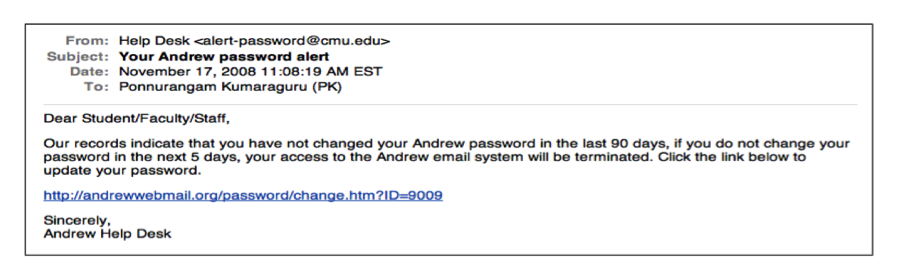
\includegraphics[scale=0.6]{gfx/kumaraguru-a}}

\quad{}\subfloat[simulated phishing website \citep{kumaraguru:2009}]{\centering{}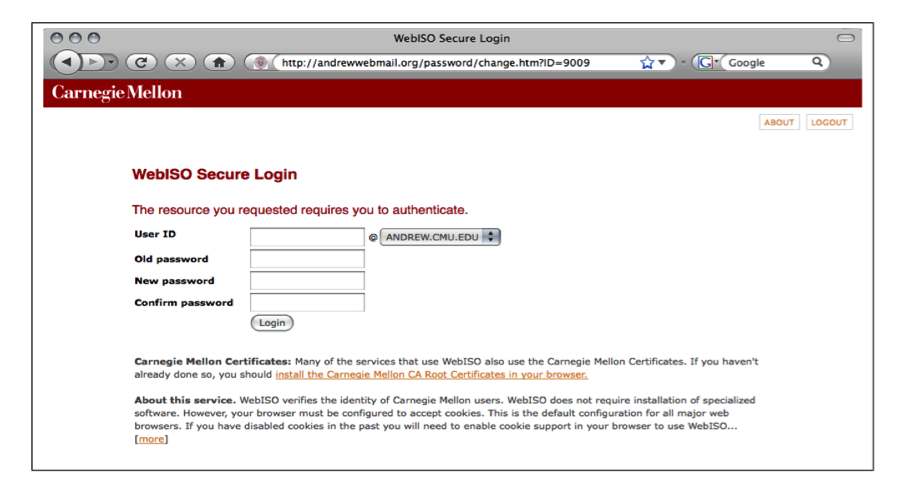
\includegraphics[scale=0.6]{gfx/kumaraguru-b}}\quad{}\subfloat[simulated phishing message \citep{kumaraguru:2009}]{\begin{centering}
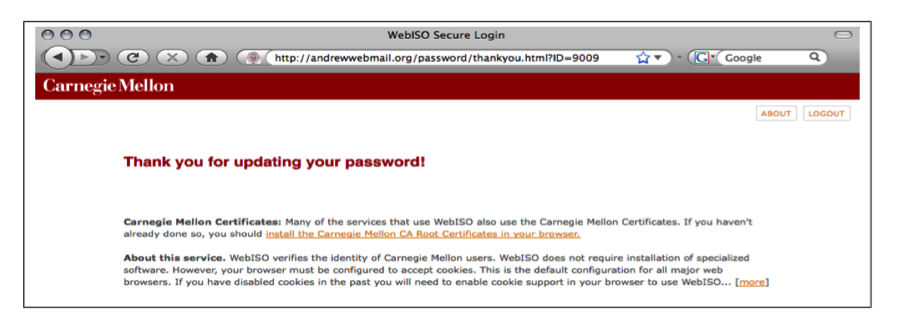
\includegraphics[scale=0.6]{gfx/kumaraguru-c}
\par\end{centering}

}\protect\caption{\label{fig:simulated}Simulated phishing attack \citep{kumaraguru:2009}}


\end{figure}


Phishguru is a security training system operated by Wombat security
technology that teaches users not to be deceived by phishing attempts
by simulation of phishing attacks\citep{phishguru}. They claimed
Phishguru provides more effective training than traditional training
as it is designed to be more engaging. \autoref{fig:em-training}
illustrates how embedded phishing training was presented by PhishGuru.

Kumaraguru, et al. investigates the effectiveness of embedded training
methodology in a real world situation \citep{kumaraguru:2009}. Evidently,
they indicated that even after 28 days after training, users trained
by PhishGuru were less likely to click the link presented in the simulated
phishing email than those who were not trained. They also find that
users who trained twice were less likely to give information to simulated
fraudulent website than users who were trained once. Moreover, they
argue that the training does not decrease the users\textquoteright{}
willingness to click on the links from legitimate emails; it means
that less likely a trained user did a false positive when he or she
requested to give information from true legitimate emails \citep{kumaraguru:2009}.
This suggests that user training strategy as an effective phishing
education in order to improve phishing awareness especially in organizational
environment.

\begin{figure}
\begin{centering}
\includegraphics[scale=0.6]{\string"gfx/phishing training\string".png}\protect\caption{\label{fig:em-training}Embedded phishing training \citep{kumaraguru:2009}}

\par\end{centering}

\end{figure}



\section{\label{sec:Human-factor-and}Human factor and persuasion}

Phishing attacks generally aim to manipulate end users to comply phisher's
request. Such manipulation in phishing attacks is achieved by social
engineering. This means that human element is tightly involved with
phishing. But how do phishers compose such deception? How come online
users are gullible to these attacks? 

Kevin Mitnick, who was obtaining millions of dollars by performing
social engineering technique, is plausibly the best known person who
had used social engineering technique to carry out his attacks. His
book that titled ``The art of deception: Controlling the Human Element
of Security'' \citep{mitnik:2001} has defined social engineering
as follows:
\begin{quote}
``Using influence and persuasion to deceive people by convincing
them that the attacker is someone he is not, or by manipulation. As
a result, the social engineer is able to take advantage of people
to obtain information, or to persuade them to perform an action item,
with or without the use of technology.''
\end{quote}
From his definition we can learn that people are the main target of
the attack, specifies some of the important tools used by the attackers,
such as influence and persuasion. 

Cialdini suggests that there are six basic principles of persuasion
\citep{cialdini:2001}, that is, the technique of making people grant
to one's request. These principles include;\textit{ reciprocation,
consistency, social proof, likeability, authority and scarcity}. Reciprocation
is \foreignlanguage{english}{the norm that obligates individuals to
repay in kind what they have received, return the favor or adjustment
to smaller request \citep{cialdini:2001}. Consistency is a public
commitment where people confirmed to commit publicly in the decision
they have made \citep{workman:2008}\citep{cialdini:2001}. Social
proof is when people follow the behavior of their peer group, role
models or important others because it is generally \textquotedbl{}fashionable\textquotedbl{}
\citep{workman:2008}. Stajano, et al. suggest people will let their
guard down when everybody around them appears to share the same risk
\citep{stajano2011understanding}. Likeability is when people giving
their trust to the people they find attractive or credible \citep{workman:2008,cialdini:2001},
when trust is achieved, compliance to grant a request may take place.
While it is our human nature not to question authority, it can be
used to cause fear, where people obey commands to avoid negative consequences
such as losing a privilege or losing something valuable, fear of punishment,
humiliation or condemnation \citep{cialdini:2001,workman:2008}. Stajano,
et al suggest that scarcity is related to time principle, that is,
when we are under time pressure to make important choice, we tend
to have less reasoning to make decision \citep{stajano2011understanding}. }

Human as the ``weakest link'' in computer security has been exists
and exploited for ages. And yet, security designers blame on users
and whine ``the system I designed would be secure, if only users
were less gullible'' \citep{stajano2011understanding}. Stajano,
et al. stated that ``a wise security designer would seek a robust
solution which acknowledge the existence of these vulnerabilities
as unavoidable consequence of human nature and actively build countermeasures
that prevent this exploitation'' \citep{stajano2011understanding}.
With this in mind, the exploration of persuasion principles is congruent
with our research goal. Cialdini's six persuasion principles will
be the foundation in our research.
